%%% LaTeX Template: Article/Thesis/etc. with colored headings and special fonts
%%%
%%% Source: http://www.howtotex.com/

\documentclass[12pt]{article}


\usepackage{apuntes-estilo}
\usepackage{fancyhdr,lastpage}
\usepackage{color,colortbl}
\usepackage{verbatim}

\def\maketitle{

% Titulo 
 \makeatletter
 {\color{bl} \centering \huge \sc \textbf{
 Administración de recursos \\ 
\large \vspace*{-8pt} \color{black} Guía básica de reconocimiento y monitoreo de recursos. 
 \vspace*{8pt} }\par}
 \makeatother


% Autor
 \makeatletter
 {\centering \small 
 	Departamento de Ingeniería de Computadoras \\
 	Facultad de Informática - Universidad Nacional del Comahue \\
 	\vspace{20pt} }
 \makeatother

}

% Custom headers and footers
\fancyhf{} % clear all header and footer fields
\fancypagestyle{plain}{\fancyhf{}}
  	\pagestyle{fancy}
 	\lhead{\footnotesize Reconocimiento y monitoreo de recursos - Departamento de Ingeniería de Computadoras}
 	\rhead{\footnotesize \thepage\ }	% ''Page 1 of 2''

\def\ti#1#2{\texttt{#1} & #2 \\ }



\begin{document}

\thispagestyle{empty}
\maketitle
\setlength{\parindent}{0pt}

\section*{Introducción}

Un administrador de sistemas es quien administra los recursos de un sistema informático. El administrador
de sistemas debe conocer cuáles son los recursos a administrar: cómo identificarlos y verificar su 
correcto funcionamiento. Durante esta guía se verán una serie de comandos y procedimientos para identificar 
recursos y verificar su estado. Dada la variedad del hardware existente hoy en día, este apunte no pretende
ser exhaustivo sino plantear un método de identificación y monitoreo a partir de ejemplos. Cunado 
el recurso a administrar no este dentro de lo visto en esta guía el administrador deberá preguntarse e
investigar cuál es la forma de identificar y observar el estado del recurso en cuestión. 

Cuando hablamos de recursos en general nos referimos a representaciones en el sistema operativo para 
recursos físicos, como por ejemplo un CPU. O bien a recursos netamente lógicos que no tienen una
contraparte física como puede ser un proceso (programa en ejecución), una prioridad de ejecución, 
un sistema de archivos, etc. 


\section*{Identificando recursos}


Comenzaremos por identificar recursos físicos, esto es listar sus características y la forma en que 
se encuentra representado en el SO. Cuando el administrador necesita realizar una tarea
sobre un recurso, por ejemplo ver si el sistema reconoce un dispositivo usb recientemente conectado, 
debe preguntarse: ¿cuál es el comando que me permite listar información acerca de este dispositivo?. 
El administrador podrá recordar un conjunto de comandos, quizá no todos, y en caso que no lo recuerde
investigará hasta encontrar la respuesta. En nuestro ejemplo del reconocimiento de un dispositivo 
usb la pregunta se resuelve casi de manera inmediata al realizar una pequeña búsqueda entre las páginas
del manual de GNU/Linux: 

\colorbox{grey}{\parbox[t]{0.95\linewidth}{ \vspace*{0.5cm} { 
Observe que efectivamente la primera y sexta línea de resultados tienen grandes chances 
de darnos algo de la información que estamos buscando (puede y de hecho lo habrá mas de un 
modo de obtener la misma información): \\ 
{\tt 
\$ man -k usb \\
lsusb (8)            - list USB devices\\
sane-find-scanner (1) - find SCSI and USB scanners and their device files\\
sisusb (4)           - SiS USB video driver\\
unetbootin (1)       - program to install Linux/BSD distributions to a partit...\\
update-usbids (8)    - download new version of the USB ID list\\
usb-devices (1)      - print USB device details\\
usb\_modeswitch (1)   - switch mode of ``multi-state'' USB devices\\
usb\_printerid (1)    - prints the ID of the printer on a USB port\\
usbip (8)            - manage USB/IP devices\\
usbipd (8)           - USB/IP server daemon\\
usbmuxd (1)          - iPhone/iPod Touch USB multiplex server daemon\\ \\
}
NOTA A PEGAR EN EL ESPEJO: ¡``{\tt man -k}'' es tu amigo!
} \vspace*{0.5cm} } } 

Obviamente si el administrador no logra resultados investigando entre las 
páginas del manual de la máquina en cuestión, irá a Internet y haciendo la consulta
correcta ``list usb devices linux'' ó ``listar usb en linux'' (en 
muchos casos la búsqueda en idioma inglés devuelva más resultados que en español),  
muy probablemente obtendrá lo que busca entre los primeros resultados: 

\begin{center}
 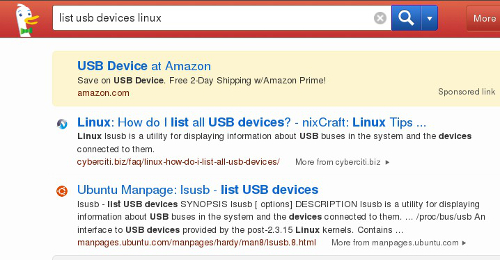
\includegraphics{lsusb.jpg}
\end{center}

Si no resuelve la pregunta de este modo, recurra a expertos en el tema, pero recuerde
intentar la identificación de recursos por sus propios medios al menos siguiendo los dos 
métodos anteriores, el administrador debe ser curioso e investigar, de otro modo puede 
obtener respuestas como esta: http://lmgtfy.com/?q=list+usb+devices+linux

\subsection*{Identificando el hardware}
En esta sección listaremos una serie de comandos clásicos para identificar recursos de
hardware dentro del sistema operativo. 

\textbf{Información del CPU:}

Si miramos el resultado de \texttt{man -k cpu}, encontraremos muchos comandos probables, quizá 
uno de los más evidentes es \textbf{\texttt{lscpu}} cuya función es listar el contenido del archivo 
\texttt{/proc/cpuinfo} (normalmente los comandos ls{\textless}algo\textgreater normalmente 
\textbf{listan} información acerca de {\textless}algo\textgreater).

El comando \textbf{\texttt{dmidecode}} tiene una sección ``Processor Information'' que muestra
información almacenada en el firmware de la placa base (SMBIOS) acerca de los componentes de 
hardware. 

\colorbox{grey}{\parbox[t]{0.95\linewidth}{ \vspace*{0.5cm} { 
{\tt
\# lscpu \\
Architecture:          i686\\
CPU op-mode(s):        32-bit, 64-bit\\
Byte Order:            Little Endian\\
CPU(s):                2\\
On-line CPU(s) list:   0,1\\
Thread(s) per core:    1\\
Core(s) per socket:    2\\
Socket(s):             1\\
Vendor ID:             AuthenticAMD\\
CPU family:            16\\
Model:                 6\\
Stepping:              3\\
CPU MHz:               800.000\\
BogoMIPS:              5586.01\\
Virtualization:        AMD-V\\
L1d cache:             64K\\
L1i cache:             64K\\
L2 cache:              1024K\\
}
El mismo resultado se obtiene ejecutando \texttt{cat /proc/cpuinfo}
} \vspace*{0.5cm} } } 

A continuación mostramos un ejemplo de la salida de \texttt{dmidecode}, en particular 
solo la sección que pertenece a información del procesador:

\colorbox{grey}{\parbox[t]{0.95\linewidth}{ \vspace*{0.5cm} { 
{\tt
\# dmidecode |sed -n '/Processor Information/,/\^\$/p'\\
Processor Information\\
	Socket Designation: Unknown\\
	Type: Central Processor\\
	Family: Phenom X2\\
	Manufacturer: AMD Corporation\\
	ID: 63 0F 10 00 FF FB 8B 17\\
	Signature: Family 16, Model 6, Stepping 3\\
	Flags:\\
		FPU (Floating-point unit on-chip)\\
		VME (Virtual mode extension)\\
		DE (Debugging extension)\\
		PSE (Page size extension)\\
		TSC (Time stamp counter)\\
		MSR (Model specific registers)\\
		PAE (Physical address extension)\\
		MCE (Machine check exception)\\
		CX8 (CMPXCHG8 instruction supported)\\
		APIC (On-chip APIC hardware supported)\\
		SEP (Fast system call)\\
		MTRR (Memory type range registers)\\
		PGE (Page global enable)\\
		MCA (Machine check architecture)\\
		CMOV (Conditional move instruction supported)\\
		PAT (Page attribute table)\\
		PSE-36 (36-bit page size extension)\\
		CLFSH (CLFLUSH instruction supported)\\
		MMX (MMX technology supported)\\
		FXSR (FXSAVE and FXSTOR instructions supported)\\
		SSE (Streaming SIMD extensions)\\
		SSE2 (Streaming SIMD extensions 2)\\
		HTT (Multi-threading)\\
	Version: AMD Phenom(tm) II N620 Dual-Core Processor\\
	Voltage: 1.5 V\\
	External Clock: 200 MHz\\
	Max Speed: 2800 MHz\\
	Current Speed: 2800 MHz\\
	Status: Populated, Enabled\\
	Upgrade: Socket S1\\
	L1 Cache Handle: 0x0001\\
	L2 Cache Handle: 0x0002\\
	L3 Cache Handle: Not Provided\\
	Serial Number: NotSupport\\
	Asset Tag: FFFF\\
	Part Number: Not Specified\\
	Characteristics:\\
		64-bit capable
}
} \vspace*{0.5cm} } } 

\textbf{Información de la memoria principal (RAM):}

\textbf{Información de dispositivos conectados a puertos PCI y USB:}

PCI y USB permiten la interconexión de dispositivos periféricos a una computadora 
personal estándar (también se encuentran en servidores junto a otro tipo de buses). 
Puede que el lector este familiarizado con la conexión de 
dispositivos USB, y con menos frecuencia PCI. Este úlimo normalmente se encuentra 
accesible dentro del gabinete donde reside la placa base, y a este tipo de buses se
conectan placas de extensión como puede ser una placa de video, de sonido, de red, etc.   

En la figura se muestran tres buses PCI para una placa base de pentium I:

\begin{center}
 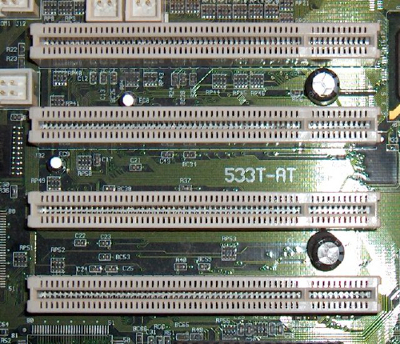
\includegraphics{Bus_pci.jpg}
\end{center}

En ambos casos (USB y PCI) suele ser de interés obtener la información de cuáles son 
los dispositivos conectados a estos puertos o buses. Convenientemente existen los 
comandos \texttt{lsusb} y \texttt{lspci}. 

Por ejemplo, si conectamos un dispositivo , digamos una memoria flash (pendrive) y 
el sistema no lo monta automaticamente como esperamos, al menos podemos listar 
 

\subsection*{Identificando recursos netamente lógicos}

\section*{Monitoreo de recursos}


\colorbox{grey}{\parbox[t]{0.95\linewidth}{ \vspace*{0.5cm} { 
{\tt 
11) none - I want to specify the time zone using the Posix TZ format.\\
\#? 1\\
}
} \vspace*{0.5cm} } } 




\section*{Licencia}

Este material es una obra derivada de los siguientes textos:

``The Clock Mini-HOWTO'' del sitio TLDP: http://tldp.org/HOWTO/Clock.html\#toc1

``The Linux System Administrator's Guide'' del sitio TLDP: http://www.tldp.org/LDP/sag/html/

\end{document}
